%%%%%%%%%%%%%%%%%%%%%%%%%%%%%%%%%%%%%%%%%
% Stylish Article
% LaTeX Template
% Version 2.1 (1/10/15)
%
% This template has been downloaded from:
% http://www.LaTeXTemplates.com
%
% Original author:
% Mathias Legrand (legrand.mathias@gmail.com)
% With extensive modifications by:
% Vel (vel@latextemplates.com)
%
% License:
% CC BY-NC-SA 3.0 (http://creativecommons.org/licenses/by-nc-sa/3.0/)
%
%%%%%%%%%%%%%%%%%%%%%%%%%%%%%%%%%%%%%%%%%

%----------------------------------------------------------------------------------------
%	PACKAGES AND OTHER DOCUMENT CONFIGURATIONS
%----------------------------------------------------------------------------------------

%\documentclass[12pt,onecolumn]{article}
\documentclass[fleqn,12pt,onecolumn]{SelfArx} % Document font size and equations flushed left

\usepackage[english]{babel} % Specify a different language here - english by default
\usepackage[square,numbers]{natbib}
% For use with natbib package
\renewcommand{\bibsection}{\section{References}}

\usepackage{sidecap}

\DeclareRobustCommand{\ion}[2]{%
\relax\ifmmode
\ifx\testbx\f@series
{\mathbf{#1\,\mathsc{#2}}}\else
{\mathrm{#1\,\mathsc{#2}}}\fi
\else\textup{#1\,{\mdseries\textsc{#2}}}%
\fi}


\def\aj{AJ}%

          % Astronomical Journal

\def\araa{ARA\&A}%

          % Annual Review of Astron and Astrophys

\def\apj{ApJ}%

          % Astrophysical Journal

\def\apjl{ApJ}%

          % Astrophysical Journal, Letters

\def\apjs{ApJS}%

          % Astrophysical Journal, Supplement

\def\ao{Appl.~Opt.}%

          % Applied Optics

\def\apss{Ap\&SS}%

          % Astrophysics and Space Science

\def\aap{A\&A}%

          % Astronomy and Astrophysics

\def\aapr{A\&A~Rev.}%

          % Astronomy and Astrophysics Reviews

\def\aaps{A\&AS}%

          % Astronomy and Astrophysics, Supplement

\def\azh{AZh}%

          % Astronomicheskii Zhurnal

\def\baas{BAAS}%

          % Bulletin of the AAS

\def\jrasc{JRASC}%

          % Journal of the RAS of Canada

\def\memras{MmRAS}%

          % Memoirs of the RAS

\def\mnras{MNRAS}%

          % Monthly Notices of the RAS

\def\pra{Phys.~Rev.~A}%

          % Physical Review A: General Physics

\def\prb{Phys.~Rev.~B}%

          % Physical Review B: Solid State

\def\prc{Phys.~Rev.~C}%

          % Physical Review C

\def\prd{Phys.~Rev.~D}%

          % Physical Review D

\def\pre{Phys.~Rev.~E}%

          % Physical Review E

\def\prl{Phys.~Rev.~Lett.}%

          % Physical Review Letters

\def\pasp{PASP}%

          % Publications of the ASP

\def\pasj{PASJ}%

          % Publications of the ASJ

\def\qjras{QJRAS}%

          % Quarterly Journal of the RAS

\def\skytel{S\&T}%

          % Sky and Telescope

\def\solphys{Sol.~Phys.}%

          % Solar Physics

\def\sovast{Soviet~Ast.}%

          % Soviet Astronomy

\def\ssr{Space~Sci.~Rev.}%

          % Space Science Reviews

\def\zap{ZAp}%

          % Zeitschrift fuer Astrophysik

\def\nat{Nature}%

          % Nature

\def\iaucirc{IAU~Circ.}%

          % IAU Cirulars

\def\aplett{Astrophys.~Lett.}%

          % Astrophysics Letters

\def\apspr{Astrophys.~Space~Phys.~Res.}%

          % Astrophysics Space Physics Research

\def\bain{Bull.~Astron.~Inst.~Netherlands}%

          % Bulletin Astronomical Institute of the Netherlands

\def\fcp{Fund.~Cosmic~Phys.}%

          % Fundamental Cosmic Physics

\def\gca{Geochim.~Cosmochim.~Acta}%

          % Geochimica Cosmochimica Acta

\def\grl{Geophys.~Res.~Lett.}%

          % Geophysics Research Letters

\def\jcp{J.~Chem.~Phys.}%

          % Journal of Chemical Physics

\def\jgr{J.~Geophys.~Res.}%

          % Journal of Geophysics Research

\def\jqsrt{J.~Quant.~Spec.~Radiat.~Transf.}%

          % Journal of Quantitiative Spectroscopy and Radiative Trasfer

\def\memsai{Mem.~Soc.~Astron.~Italiana}%

          % Mem. Societa Astronomica Italiana

\def\nphysa{Nucl.~Phys.~A}%

          % Nuclear Physics A

\def\physrep{Phys.~Rep.}%

          % Physics Reports

\def\physscr{Phys.~Scr}%

          % Physica Scripta

\def\planss{Planet.~Space~Sci.}%

          % Planetary Space Science

\def\procspie{Proc.~SPIE}%

          % Proceedings of the SPIE

\def\rmxaa{Rev.~Mex.~de~A\&A}

\let\astap=\aap

\let\apjlett=\apjl

\let\apjsupp=\apjs

\let\applopt=\ao

%

\uchyph=0

%\newcommand{\KM}[1]{\textcolor{purple}{#1}}
%\newcommand{\vlk}[1]{{\color{blue}{#1}}}


%----------------------------------------------------------------------------------------
%	COLUMNS
%----------------------------------------------------------------------------------------

\setlength{\columnsep}{0.55cm} % Distance between the two columns of text
\setlength{\fboxrule}{0.75pt} % Width of the border around the abstract

%----------------------------------------------------------------------------------------
%	COLORS
%----------------------------------------------------------------------------------------

\definecolor{color1}{RGB}{0,0,90} % Color of the article title and sections
\definecolor{color2}{RGB}{0,20,20} % Color of the boxes behind the abstract and headings

%----------------------------------------------------------------------------------------
%	HYPERLINKS
%----------------------------------------------------------------------------------------

\usepackage{hyperref} % Required for hyperlinks
\hypersetup{hidelinks,colorlinks,breaklinks=true,urlcolor=color2,citecolor=color1,linkcolor=color1,bookmarksopen=false,pdftitle={Title}}

%----------------------------------------------------------------------------------------
%	ARTICLE INFORMATION
%----------------------------------------------------------------------------------------

\JournalInfo{ASTROPHYSICS DATA ANALYSIS: S/T/M} % Journal information
%\Archive{Additional note} % Additional notes (e.g. copyright, DOI, review/research article)

\PaperTitle{Getting more out of archival X-ray spectra: New spectral fitting methods}
\Archive{}

\Authors{}
%\affiliation{*\textbf{Corresponding author}: hgunther@mit.edu} % Corresponding author

\Keywords{Astrophysical Databases, Interstellar Medium and Star Formation} % Keywords - if you don't want any simply remove all the text between the curly brackets
\newcommand{\keywordname}{Keywords} % Defines the keywords heading name

%----------------------------------------------------------------------------------------
%	ABSTRACT
%----------------------------------------------------------------------------------------


\Abstract{}

\begin{document}



\flushbottom % Makes all text pages the same height

\maketitle % Print the title and abstract box
%\tableofcontents % Print the contents section

\thispagestyle{empty} % Removes page numbering from the first page

\setcounter{tocdepth}{1}
\tableofcontents

%----------------------------------------------------------------------------------------
%	ARTICLE CONTENTS
%----------------------------------------------------------------------------------------
%\newpage


\section{Introduction}
Data taken with space telescopes is necessarily resource limited. Building and operating space telescopes is expensive, and there always are more ideas for worthwhile investigations than there is observing time as seen in the large oversubscription factors for XMM-Newton, Chandra, and others. Therefore, it is imperative to make the most out of the data that we have in the archives and to continuously innovate in the data reduction and fitting processes to learn as much as we can.

Yet, the backbone of X-ray spectral fitting today is essentially the same as it was even before the launch of XMM-Newton and Chandra.

\section{Objectives}
Our main objective in this proposal is to develop methods and software to obtain a higher signal-to-noise ratio (SNR) from existing, archival X-ray spectra by developing improved spectral fitting algorithms which make use of more information (such as the cross-dispersion profile for a grating spectrum or temporal changes in the background rate) than the current state-of-the art algorithms. By using this additional information, source photons that are currently discarded can be used in spectral fitting and thus parameters of physical models can be constrained better.

We will demonstrate those methods with an analysis for the X-ray emission from a young Herbig Ae/Be star, where we will test if the soft X-ray component traces a jet collimation shock or if it is coming from close to the star itself (corona or accretion shock).

\textbf{We stress that the methods are fully general and can be used for any type of X-ray spectrum}, from young stars, to accreting neutron stars, to spectra of full clusters of galaxies, both grating spectra and CCD-level spectra. However, for the sake of this discussion, we pick shocks in young stars as an example and show how the improved data analysis procedures will address fundamental open questions in star formation.

\subsection{Main objective: Better signal from existing data}
For decades, NASA has invested enormous financial, logistical, and technical resources into X-ray space missions. The biggest of those are NASA's great observatory Chandra and the ESA-lead XMM-Newton mission, both operating in their 25th year. A fleet of smaller missions, such as Swift, NuSTAR, NICER, IXPE, and others supplement this legacy. % and archival data is also available for earlier missions with NASA involvement such as BeppoSAX and ASCA.
Taken together, the data archive of X-ray observations maintained by NASA's HEASARC is a treasure trove of information about the high-energy universe.
The stated goal of the ADAP program is to ``to capitalize on
this [meaning: archival data] invaluable asset and enhance the scientific return on NASA mission investments''.

The current methods of analyzing X-ray spectral data are not optimal, in the sense that they discard information for the sake of computational efficiency and easier standardization of data products. \textbf{We propose to develop new methods that will allow us to extract more information from the same data, thus increasing the scientific return on the investment into the X-ray missions.}

%\objectivebox{Objective 1 (general)}{Improve the signal-to-noise ratio in X-ray spectra compared to the current standard spectral fitting algorithms.}

\begin{figure}
    \includegraphics[width=0.33\textwidth]{rgs1_pi}
    \includegraphics[width=0.33\textwidth]{rgs1_xdisp}
    \includegraphics[width=0.33\textwidth]{rgs1_bkg}
    \caption{Data from an XMM-Newton grating observations (RGS1 in ObsIDs 0502370201)
    \emph{left:} CCD energy vs. wavelength (from the detector position). Blue regions mark the detector energies where 90\% of the source photons are expected. The green region marks photons from a calibration source.
    \emph{middle:} Spectral image with the dispersed spectrum running left to right (showing only photons within the blue region of the left panel), zoomed into a region with strong emission lines. The source extraction region (blue) contains 66\% of the cross-dispersion profile. The black lines mark the boundaries of the 98\% cross-dispersion profile, which is much wider and dominated by background counts.
    \emph{right:} Background light curve. The red dashed line shows a typical value for background filtering: All times when the background rate is higher (gray bars) are discarded. In this observation that is only a small fraction of the time, but in many XMM-Newton observations background is stronger.
    \label{fig:rgs1}}
\end{figure}

Developing a truly ``optimal'' fitting process that takes all possible information into account and works robustly for all types of X-ray spectra is a very ambitious goal because many aspects of this would require new calibrations. While it might be possible to derive most of that from existing archival calibration data, that is far beyond the scope of this proposal. We will concentrate on just three aspects which are particularly impactful for data from the XMM-Newton reflection grating spectrometer (RGS) and that can be implemented with calibration data that is already available: the cross-dispersion profile, the order sorting using CCD energies, and the background rate (Fig.~\ref{fig:rgs1}). While we will develop a framework that can be extended to other aspects (section~\ref{sect:impact_other}), we leave that to future work. \textbf{The main objective of this proposal is to provide practical, tested, and documented open-source software to the community that can be used for XMM-Newton grating spectroscopy and that reduces the uncertainties of fitted spectral parameters compared to standard methods.}

%\objectivebox{Objective 1 (detail)}{Significantly improve the signal-to-noise ratio in spectral modelling of XMM-Newton grating data by using the cross-dispersion profile and temporal changes in the background rate.}


\subsection{Secondary objective: Shocks in the jet collimation and accretion for young stars}
Our secondary objective is to determine if the soft X-rays in intermediate stars originate in a jet collimation shock similar to CTTS. This is described in more detail in section~\ref{sect:application} after we explain the methods we will develop in this proposal.

\newpage

\section{Impact}

\subsection{Better signal from XMM-Newton grating data}
Observations with high background stand to profit more from our new method than observations where the source signal dominates. However, as observers tend to propose for the most extreme (the youngest, the lowest mass, unusual abundances) sources that are feasible to observe and minimize exposure times until just sufficient to reach scientific goals, many datasets are in the regime where better fitting methods can make a significant difference.

In most XMM-Newton observations  all detectors are operating, even if there is no point source at the aimpoint; thus we cannot simply count the number of XMM-Newton/RGS datasets to determine the number of observations that our new method will improve. However, the Browsing Interface for RGS Data (BiRD) assigns a quality from 0 to 10 to all archival RGS spectra. %, where 0 means that no photons are detected and 10 that photons are detected in every spectral bin. This is a rough measure since absorbed sources will naturally lack signal at long wavelength, but can deliver highly impactful science and a large count number could also be caused by high background.
The data presented in Fig.~\ref{fig:rgs1} that will be reanalyzed in this program to achieve objective 2 is listed as quality 3 in BiRD. There are about 1800 spectra of comparable quality (2-4) in BiRD and over 3000 that are significantly better (quality 5-10). Together, that makes almost 5000 RGS datasets that will immediately benefit from the software we develop in this program. Of course, not all this data will be republished and the improved signal-to-noise ratio alone will not lead to new scientific results in every case. On the other hand, there are cases where new types investigations become possible, for example in observations with frequent background flaring it is difficult to look for spectral changes after removing time intervals with a high background; in contract our new method would allow to make use of all times.


\subsection{Better signal from any X-ray grating or CCD-level spectrum}
\label{sect:impact_other}
%In this program we will develop a new method to fit XMM-Newton grating spectra that makes use of the information in the cross-dispersion profile and the background light curve.
There are several other aspects that the same method can be extended to, it just requires extra work beyond the scope of this proposal. However, results of this proposal will prove the value of this approach to the community and the code that we provide as part of this project will make it easier to treat other aspects in the future making it a lot more likely that other researchers, a follow-up ADAP program, or instrument support groups in e.g.\ the \emph{Chandra X-ray Center (CXC)} or the \emph{XMM-Newton Science Operations Center (SOC)} will pick up the work and extend it.

\begin{figure}
    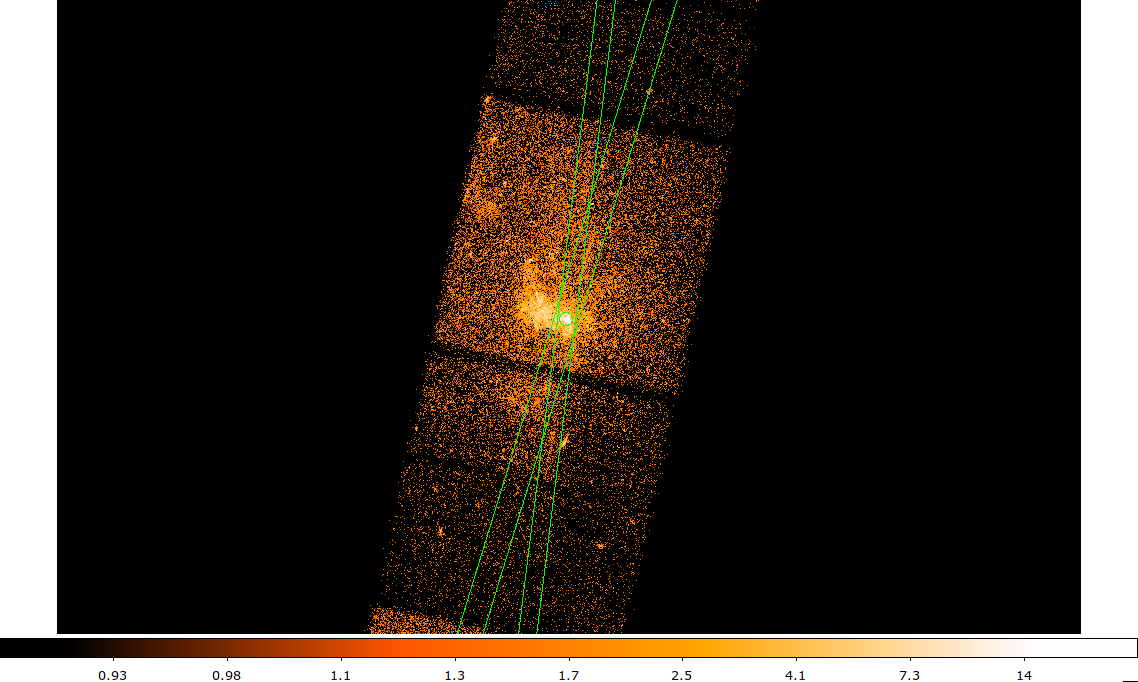
\includegraphics[width=0.5\textwidth]{SgrAstar}
    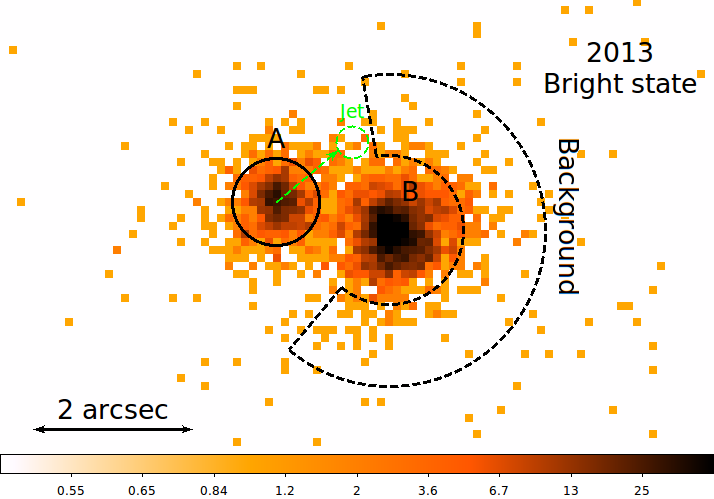
\includegraphics[width=0.5\textwidth]{schneider_2015}
    \caption{
        The general methods we develop can be used for all X-ray data. This figure shows two examples.
        \emph{left:} Chandra observation (from archival ObsID 13842) of Sgr~A\* with the HETG. The green boxes show the extraction region for the HEG and MEG; they include significant diffuse emission and a few point sources. The color bar shows the number of counts per bin.
        \emph{right:} RW~Aur~A (left) and B (right) are close enough that their PSFs partially overlap. The extraction region for RW~Aur~A is chosen to be small to reduce that contamination at the cost of discarding source photons from the star. The color bar shows the number of counts per bin. From: \cite{2015A&A...584L...9S}\label{fig:other_uses}}
\end{figure}

X-ray data contains a wealth of information about every single photon, while the extracted spectrum only lists the number of counts per spectral (energy) bin. Any aspect discarded in that binning could improve the constraints on spectral models, for example:
\begin{description}
    %\item[order-sorting] In grating spectra, the intrinsic energy resolution of the CCD is used to see determine the order of a photon, e.g.\ if the photon energy matches $m\lambda$ for order 1 or 2, or falls in between orders and thus must be a background photon to be discarded. This is exactly analogous to the cross-dispersion profile, where photons close to the expected value are more likely to be source photons than photons far away and the fitting algorithm should take that into account instead of a binary decision to include or exclude a photon.
    \item[cross-dispersion in Chandra/HETGS or LETGS] It will be straightforward to apply the same method we develop for XMM-Newton/RGS spectroscopy to Chandra/HETGS or LETGS data (Fig.~\ref{fig:other_uses}, left). %The gain in signal-to-noise ratio will be lower, because the cross-dispersion profile is much narrower in Chandra data, and thus we concentrate on XMM-Newton data in this proposal. However, there are specific datasets where the background is problematic for spectral extraction even in Chandra/HETGS data (for example, observations of the galactic center or in star forming regions where many point sources and a diffuse background can contaminate the dispersed spectrum, see Fig.~\ref{fig:other_uses}, left).
    \item[Accounting for the PSF in CCD imaging] Similar to how we can use the cross-dispersion profile in a grating spectrum, we can use the point spread function (PSF) in CCD imaging to weight the photons in the fitting process instead of simply excluding all photons beyond a certain radius. %A more sophisticated fitting algorithm could use the PSF information to weigh the photons in the fitting process in some way because photons in the center are more likely to be source photons than photons at the edge of the PSF.
    \item[overlapping sources in CCD imaging] An extension of the PSF weighting would be to account for overlapping sources, e.g.\ Fig.~\ref{fig:other_uses} (right). The extraction region for RW~Aur~A is chosen to be small to reduce that contamination at the cost of discarding source photons from the star. Fitting both source spectra and the background simultaneously and using the position of each detected photon relative to the two sources would allow us to include all photons in the fitting and thus improve the constraints on the spectral model. This is a somewhat different approach than \cite{2015ApJ...808..137J}, who used a Baysian statistic to separate photons between sources, but did not fit physical spectral models.
    \item[event grade/pattern] The charge cloud from a single photon is detected in more than one pixel in the CCD. That shape is encoded in the ``grade'' or ``pattern''. Photons of specific grades/patterns are more likely to be background events than others. Yet, in standard fitting a grade/pattern filter is applied and photons are either included or excluded. A more sophisticated fitting algorithm could use the grade/pattern information to weigh the photons in the fitting process.
\end{description}



\subsection{Future observations}
This proposal is focussed on archival data, but if the approaches we develop here are successful, future proposerscan accomplish their scientific goals with fewer X-ray counts, enabling them to reach further with existing facilities. This could mean proposing for shorter exposure times, such that more different investigations can be accepted in any given cycle, or reaching for targets that are otherwise too far away or too extincted to be observed.

\section{Relevance to Program Element}
The purpose of the ADAP is to increase the return on NASA's investment into decades of space astrophysics missions through the analysis of archival observations. This proposal is doing exactly that. We are going to focus on XMM-Newton/RGS data that has been in the public archive for many years, and XMM-Newton is explicitly listed as one of the missions targets by he ADAP.
The call for the ADAP also explicitly explains for the scope for new software:
\begin{quote}
    An essential component of any activity funded under the Astrophysical Databases
research area of the ADAP is the ultimate dissemination of high-value data products
and data analysis tools to the astronomical community.
\end{quote}
Our two objectives are to develop a new spectral fitting algorithm and to apply it to a specific science case; both objectives directly target the goal and scope of ADAP.

\section{Technical Approach and methodology}

The basic idea we propose is similar to the ``optimal extraction'' algorithm for CCD spectroscopy \cite{1986PASP...98..609H} that is widely used in the optical and IR. The ``optimal extraction'' is optimal in the sense that it achieves the maximum possible SNR for the extracted spectrum, given the signal and background in the observed data. In that algorithm, data is not simply summed up along the cross-dispersion profile, but it uses a weighted sum where the weight for each pixel depends on the position in the cross-dispersion profile. Pixels in the well-exposed center of the cross-dispersion profile have a higher weight than those in the wings. The algorithm we propose to develop will also make use of the information in additional dimensions (cross-dispersion profile, CCD energy, background rate). In X-rays we are usually in a regime of few counts, where we need to track individual photons so that the fit can be done using proper Poisson statistics. In contrast, the algorithm from \cite{1986PASP...98..609H} is based on the assumption that the noise is Gaussian which would lead to significant systematic biases of the fitted parameters in a low-count regime \cite{1989ApJ...342.1207N,1996NIMPA.372..289J,1999ApJ...518..380M,2001NIMPA.457..384H}. Even when correcting for this effect through e.g.\ the Neyman's $\chi^2$ \cite{1999ApJ...518..380M}, physical results like galaxy cluster scaling relations are expected to by systematically shifted by 5-10\% \cite{2009ApJ...693..822H}. Only a true Poisson likelihood maximization can avoid this bias \cite{1979ApJ...228..939C,2007A&A...468..501A} hence the need for a similar, but different new algorithm. \footnote{In practice, maximizing the Poisson likelihood is usually implemented as minimizing the negative log likelihood, which is mathematically equivalent and numerically easier to evaluate.}


\subsection{State of the art and data standards in X-ray spectroscopy}
The need for preserving the Poisson statistics has historically driven the data formats and fitting programs that are used in X-ray astronomy.
Unlike optical spectroscopy where many facilities exist, in X-ray spectroscopy there have been just about a dozen X-ray observatories in the history of astronomy. This invites a common standardization of data formats, formalized in the early 1990's by the
Office for Guest Investigator Programs (OGIP), then a division of the
Laboratory for High Energy Astrophysics at Goddard Space Flight Center. These standard file formats for spectra and the required calibration data have
since been used for essentially every high-energy astrophysics mission
world-wide.
%The activities of that group have been taken over by the HEASARC
%FITS Working Group (HFWG). %\footnote{\url{https://heasarc.gsfc.nasa.gov/docs/heasarc/ofwg/ofwg_intro.html}}.
The standard is very stable with only a few minor additions in the last 25 years. In OGIP terminology, there are three ingredients to a spectral fit: the spectrum (PHA file) \cite{PHA}, the detector response (ARF file), and the energy-dependent line-spread function (RMF file) \cite{RMFARF}.

With this proposal, we want to improve spectral fitting algorithms, which will allow us to fit more detailed models with more parameters to the same data or to better constrain physical parameters. Before we can explain our proposed work, we summarize the current OGIP paradigm of fitting (see \cite{2011hxra.book.....A} for a full review or \cite{2023hxga.book..150B} for a more practical introduction), so that we can show how our approach is better.
The spectrum (pulse-height amplitude (PHA) file, referring to the height of electronic pulses from the detector) contains the number of photons per energy bin.
%The same formalism is used both for dispersed grating spectra and for spectra from imaging X-ray detectors with intrinsic energy resolution (CCDs and microcalorimeters) that measure the energy of each incoming photon and thus we can take the list of photons detected from one source and bin the photons into ``energy channels'' in a PHA file.

In order to predict the count number for any given physical model we need to consider instrumental effects, such as the
mirror size, and the grating and CCD efficiency. Clearly, we do not want to
work all those details into each and every physical model. Instead,
OGIP defines the ARF, which is essentially a table of ``effective area''
vs. wavelength.
For grating spectra, the signal is summed along the cross-dispersion direction
and thus the value of the ARF for each wavelength is essentially the product of
mirror effective area, grating efficiency, and the sum of the pixel
efficiencies.
%In this way,
%effects like pixel-to-pixel efficiency differences or detector dead time are
%taken into account.

For X-ray detectors, the line-spread-function (LSF) usually varies widely with wavelength; sometimes the line width can differ by a factor of a few between one end of the detector and the other. So, we do need an LSF that depends on energy/wavelength. The shape is also often complex with wide wings (scattering on the mirror can move photons far from the expected position in a grating spectrum) and secondary peaks (e.g.\ due to electron escape peaks in the silicon layer of a CCD).
In the OGIP formalism, this is done with a response
matrix.
%In principle,
This is a matrix, where each element $R_{ij}$
describes what fraction of the true flux at wavelength $\lambda_j$ is detected
at $\lambda_i$.
%(In practice, the matrix might not be square if either
%$\lambda_i$ or $\lambda_j$ are oversampled. Also, most elements of this matrix are close to zero
%and memory usage is optimized by not storing the entire matrix.)

When using Poisson statistics, the background cannot be subtracted, because the
difference between two Poisson distributions is \emph{not} a Poisson
distribution. Instead, we extract a count spectrum from the background region
and fit a background model separately. The background model need
not be physical, it can just be e.g.\  a polynomial. When we fit the source
model, we construct our model $m$ as the sum of the background model (scaled to
the correct extraction area, e.g.\ 0.25 times the polynomial if the background
region is four times the source extraction region) and a physical model for
the source (e.g.\ a black-body plus extra emission lines).

Following \citet{1979ApJ...228..939C} we want to minimize the following statistic:
\begin{equation}
C = 2\sum_{i=1}^n m(\lambda_i) - N_i \ln(m'(\lambda_i))
\label{eqn}
\end{equation}
where the $N_i$ is the number of counts in bin
$i$ and $m'$ is the model normalized to give the number of counts (not the flux).
%Today, bmore often a
%slightly modified version of this statistic is used which converges to the
%familiar $\chi^2$ statistic for large $N_i$:
%\begin{equation}
%C = 2\sum_{i=1}^n m'(\lambda_i) - N_i + N_i \ln(N_i/m'(\lambda_i))
%\label{eqn}
%\end{equation}

A number of spectral fitting packages have been developed
that read PHA, ARF, and RMF files and perform spectral fitting by forward-folding a physical source model through the instrument response.
The
most popular of these programs is XSPEC \citep{1996ASPC..101...17A}, but Sherpa
\citep{2001SPIE.4477...76F}, ISIS \citep{2000ASPC..216..591H}, or SPEX
\citep{1996uxsa.conf..411K} have $>300$ citations each, indicating that these
programs are used by a large community, too.


\subsection{Information is lost in OGIP PHA files}
As it stands, the OGIP scheme of spectra in PHA files, and instrumental information in ARF and RMF files (possibly supplied as a combined file by the data pipeline) is an overwhelming success story. Spectral data from essentially all X-ray observatories can be analyzed interchangeably with the same code and the same analysis settings, and new theoretical models can be coded and supplied to the community in a single form. Moreover, the PHA, ARF, and RMF files are designed to be efficient in file size. Even joint fits of many spectra can often be done comfortably on a laptop; the run-time is usually dominated by evaluation of the spectral model, not by forward-folding with the ARF and RMF and calculating the fit statistic.


\textbf{Yet, binning photons into a PHA file inherently causes information loss. That information loss means that we throw away valuable observation time since we need longer observations to reach the same signal-to-noise ratio.}

The fundamental issue is that a photon is either in the extraction region (source or background), or it is not. However, the boundary between ``in the source region'' and ``outside the source region'' is arbitrary. For an imaging observation, one might choose to extract 90\% of the PSF as the source region or 75\% of the PSF or some other number; there is no real statistical basis why one is better than the other. Similarly, for a grating spectrum, one could extract 66\% or 77\% or 90\% or some other fraction of the cross-dispersion profile.

In grating spectra, filtering is done in three dimensions: the photon energy as measured by the CCD, the cross-dispersion profile, and the background rate. The \textbf{CCD energy} is used to sort the photons into orders, discarding photons where the CCD energy does not match the expected energy for a photon at that position in the diffraction order (Fig.~\ref{fig:rgs1}, left). Yet, limited CCD energy resolution means that a region containing 90\% of the source photons will also contain some background photons. In the standard analysis, all photons in that region are included in the extracted spectrum and all photons outside are discarded.

The PSF or the \textbf{cross-dispersion profile} are typically peaked with wide wings. Thus, an extraction region containing 66\% of the source photons will be narrow with relatively low background, but it throws away a third of the photons. On the other hand, e.g.\ a 98\% extraction region contains almost all the source photons, but is so large that the number of background photons included drowns out important spectral features (Fig.~\ref{fig:rgs1}, middle, where blue boxes include the 66\% of the source photons, and black lines mark the outer boundary of the much larger 98\% cross-dispersion profile).

Similarly, the photon is either observed at a time of low \textbf{background} and is included in the extracted spectrum, or it is observed at high background and is excluded. Yet, Fig.~\ref{fig:rgs1} (right) shows that, again, the boundary is somewhat arbitrary. A photon observed at a background rate of 0.1001~cts/s is not fundamentally different from a photon observed at 0.0999~cts/s, yet the latter is included in the spectrum and the former is not.

\textbf{We need to move beyond a binary choice of photons in- or excluded.} When we do that, we can have our cake and eat it, too. A photon that is detected in the peak of the PSF or cross-dispersion profile is most likely a source photon, a photon much further out is less likely to be a source photon and more likely to be a background photon; similarly a photon detected at a time of low background is more likely to be a source photon than a photon detected at high background. In this proposal, we will concentrate on RGS spectra and use the additional dimensions ``cross-dispersion'', ``CCD energy'', and ``background rate'', but in principle the same can be done with other dimensions that include additional information about how likely it is that a photon is a source photon, e.g.\ the grade/pattern or the distance from a source in an image.

%\subsection{Fitting with additional dimensions}

\subsection{Software implementation}
XMM-Newton data reduction is done with the SAS (Science Analysis System) software, which can be controlled from the command line or through Python wrappers. We will use the latter option to script the required data reduction scripts.

Fitting and modelling will be done with the Sherpa \cite{2001SPIE.4477...76F} software. On the one hand, Sherpa interfaces to the XSPEC model library, providing the vast majority of relevant X-ray spectral models. Sherpa reads PHA and ARF/RMF files, and performs forward folding; on the other hand, Sherpa also already has build in functionality for 2D and higher dimensional fits. Since Sherpa is implemented in Python with speed critical routines in C++, it is relatively easy to combine existing model classes into the 2D and higher dimensional models we need here.


\section{Uncertainty/Risk and mitigation}
\label{sect:risk}
There are two main risks in this proposal: The first is that the method suggested only leads to small incremental gains in the SNR ratio, the second is that instrumental effects such as hot columns, dead pixel and non-uniform backgrounds make the method hard to use in practice or numerically unstable in the fitting process.

We address these risks by developing two different numerical methods and also spending time to address aspects of the problem analytically (see work plan). From those options, we will choose the method that works best in practice. So, failure of any one approach will not impede the success of this proposal. Here, we show two simple prototypes for one of the three dimensions we will use in the proposal (cross-dispersion profile) to demonstrate the potential of the method; \textbf{if all three dimensions (cross-dispersion, CCD energy, background rate) were added, the relative gain in SNR would be roughly cubed compared to what is seen in these simple examples.}
%designed to match a typical situation but with reduced complexity (e.g.\ we simulate only a small part of the detector, such that the cross-dispersion profile is constant, the background is flat, and there are no hot columns or chip gaps).

\subsection{Approach 1: 2D fitting}

We simulate a single emission line at 21.6~\AA{} with 20 photons on a background of 40 photons in the range 21.4 to 21.8~\AA{} (Fig.~\ref{fig:toy2d}, left). For simplicity of the code implementation, we pick a Gaussian profile in dispersion and cross-dispersion profile. The true XMM-Newton profiles are peaked like Gaussians but have wider wings. The true cross-dispersion profile is well known from calibrations, so this is easy to switch out. We then fit a 2D model with a fixed width in dispersion and cross-dispersion direction. We also extract a traditional 1D spectrum from the blue region in Fig.~\ref{fig:toy2d} (left) and a 1D background from the gray region. We repeat this simulation 1000 times and fit the 2D model to each of the simulated datasets and the 1D model to each of the extracted 1D spectra plus 1D background. Figure~\ref{fig:toy2d} (left) shows one simulated dataset and figure~\ref{fig:toy2d} (middle and right) shows the distribution of the fitted values for the number of photons in the line and the location of the line. The line position is recovered accurately, but the 1D fit shows an offset from the true value for the flux and a spread in the fitted values about 30\% larger than the 2D fit. %While the exact numbers depend on the number of counts in the line and the background and the width of the chosen extraction region, this simple simulation clearly shows the potential of the multidimensional fitting approach.
The gain in SNR from each added dimension is roughly multiplicative, so adding three dimensions (CCD energy, cross-dispersion, background rate) instead of one, would reduce error bars by about $1.3^3=2.2$ compared to the 1D fit - a significant improvement.


%%% 3D


\begin{figure}
    \includegraphics[width=0.5\textwidth]{dummy2dimage}
    \includegraphics[width=0.5\textwidth]{dummy2vilin}
    \caption{\emph{left:} Simulation of photons for a single emission line on background. The true line position is at 21.6~\AA{}. Yellow bins have one photon per bin, red two photons, and black three photons. In the 2D approach, we fit a 2D model with fixed width in dispersion and cross-dispersion direction. For comparison, we also extract a traditional 1D spectrum from the blue region and a 1D background from the gray regions (compare to Fig.~\ref{fig:rgs1}). \emph{middle, right:} Distribution of the fitted values for the number of photons in the line (scaled for the limited extraction region in the 1D case) and the location of line from 1000 simulations. The true values are marked with black lines.The 2D fit is clearly superior in determining the line flux.
    \label{fig:toy2d}}
\end{figure}


\subsection{Approach 2: Multiple 1D fits}

An alternative approach is to keep the data formats closer to the OGIP standard and make more use of the standard instrument pipelines. Using standard SAS procedures, we extract data covering 50\%, 75\%, 90\%, 95\%, and 98\% of the cross-dispersion profile simply by setting the \texttt{xpsfincl} parameter in the standard SAS task \texttt{rgsproc}. The PHA files have a column \texttt{COUNTS} that contains the counts per spectral bin. We simply subtract the counts of an inner region from the counts of an outer region, such that we get PHA files covering 0-50\%, 50-75\%, etc.\ of the cross-dispersion function. Similarly, we subtract the responses to get the effective area in the 0-50\%, 50-75\%, etc.\ regions. Leveraging Sherpa tools to read and write those files, this can be done in $<100$~lines of Python code. This way, we obtain 5 statistically independent spectra for each observation that we can fit simultaneously with the same physical model for the source and a model for the background that is scaled to the physical size of the detector region for each part.

This approach makes better use of existing pipeline and fitting tools (requiring less new code development and taking hot columns, CCD gaps etc.\ into account by using standard instrument pipelines) and is analogous to what users already do (in XMM-Newton analysis, spectra from the PN, MOS1, MOS2, RGS1, and RGS2 are often fit simultaneously with the same physical model), but it is also less flexible and scalable. In our prototype, we used five regions for the cross-dipsersion direction, with three extra dimensions we would already have $5^3=125$ regions.

\subsection{Risk assessment}

Compared to just summing up all pixels in the source region, an ``optimal extraction'' that makes use of the cross-dispersion profile gives the same SNR improvement as increasing the exposure time by 70\% for background-limited spectra \cite{1986PASP...98..609H}. Our prototype shows a similar improvement. Thus, we are confident that the methods and software to be developed in this program will significantly improve the SNR in fitting XMM-Newton/RGS spectra. Instrumental effects such as the change of the cross-dispersion profile with wavelength, hot columns, dead pixels, or non-uniform background are all already treated in the traditional extraction of PHA/ARF/RMF files. Dealing with them in 2D is not fundamentally difficult, it just requires grabbing the right information from the calibration files and implementing it in the 2D fitting. We are confident that we can do that, given sufficient time (see work plan).

We also limit risk by limiting the scope of this proposal to just developing the core method for XMM-Newton/RGS data and applying it to single science case; we will leave implementation for other instruments and other data dimensions listed in section~\ref{sect:impact_other} to future work.

\section{Application to young stars}
\label{sect:application}
\subsection{Secondary objective: Shocks in the jet collimation and accretion for young stars}
Stars form when large clouds of gas and dust contract under gravity. While the initial infall is radial, conservation of angular momentum quickly leads to the formation of an accretion disk. These disks are the sites of planet formation. Over time the disks disperse through winds, accretion onto the forming planets, and accretion onto the star itself. This takes a few Myr for low-mass stars with $M_* < 3\; M_\odot$, less time for star of intermediate mass, and high-mass stars evolve so quickly that they are still deeply embedded in the native cloud at this stage, so details are invisible. Many young low-mass and intermediate stars also drive powerful outflows, which are usually layered \cite{2000ApJ...537L..49B}. The outermost layers are launched magnetocentrifugally from the disk and are relatively slow (a few km/s to 10's of km/s) and cool. The inner layers are the faster and hotter and are launched at smaller and smaller radii, deeper in the gravitational well; the innermost component can be a highly collimated jet. However, it is unknown how those jets are launched, where exactly the mass comes from, and how they are collimated.

There are a few cases where the innermost layer is hot enough to be seen in X-rays (e.g. \cite{2005ApJ...628..811S,2008A&A...478..797G}, see also \cite{2022hxga.book...57S} for a review), presumably heated by shocks with speeds $>300$~km/s. In the classical T~Tauri star (CTTS) DG~Tau, three different X-ray components are spatially resolved \cite{2008A&A...488L..13S,2011ASPC..448..617G}: The stellar corona, an inner component about 30~au from the star, and an outer, shock-heated component. In CTTSs, that inner shock component has been modeled as a ``diamond'' recollimation shock \cite{2016A&A...596A..99U} or as a recollimation shock driven by the thermodynamic pressure of the much denser, outer layers of the outflow \cite{2014ApJ...795...51G}. CTTS are cool enough to have convective envelopes and generate strong magnetic fields, which connect the star to the disk and probably cause that jet collimation in some way.
Intermediate mass stars are not expected to operate a solar-type dynamo. However, magnetic fields are detected in some of them, possibly due to small-scale turbulent dynamos or fossil fields swept up in the initial accretion process. If the jet collimation is magnetic, the different magnetic fields should lead to different jet collimation processes.
\textbf{We will determine if the soft X-rays in intermediate stars originate in a jet collimation shock similar to CTTS.}

\subsection{Impact}
How jets are launched and collimated is a fundamental question in star formation that determines how young stars interact with their environment, how the mass accretion rate onto the star is regulated, and how the magnetic fields of the star and the disk interact. Only X-ray data can answer these questions for the fastest jet component, because in all other wavelengths the signal is dominated by the slower, more massive jet components.
Only very few intermediate-mass stars with an accretion disk are within 150~pc, where they are easily observable with X-ray grating spectroscopy. Of those, only HD~163296 has a known X-ray jet. Thus, our proposal to improve the fitting methods and make the most of the existing data is the only alternative to new, deeper observations of this source.
%Increasing the limit on the distance between star and X-ray emission region by reducing error bars will rule out a coronal origin of the X-ray emission and thus firmly establish the presence of a collimation shock; alternatively, if the best-fit value moves closer to the star with the improved analysis, it will show that the X-ray emission is coronal in origin.

\subsection{Technical Approach and methodology}
A jet collimation shock is offset from the central star, possibly by many au, but at the very least by a few stellar radii. Thus, simply determining the location of the soft emission is enough to decide if it originates in a jet collimation shock. If it is located on the star, is must be coronal or formed in an accretion shock, if it is offset from the star, it is coming from a jet collimation shock. Unfortunately, HD~163296 does not show spatial offsets between soft and hard (stellar) X-ray emission in imaging. However, spectral information can be used. In particular, one can measure the ratio between the forbidden ($f$) and the intercombination ($i$) line in the He-like triplet of O~{\sc vii}. This $f/i$ line ratio is sensitive to the density and the UV field in the emission region \cite{2001A&A...376.1113P}, since either collisional or photo-excitation can alter the populations of the upper levels.
This measurement has been attempted in the young, intermediate mass stars AB~Aur \cite{2007A&A...468..541T} and HD~163296 \cite{2009A&A...494.1041G}. In HD~163296, the result is marginal: The 90\% confidence region for the location of the shock excludes the stellar surface (i.e.\ an accretion shock) but reaches as far down as $0.7\;R_\odot$ above the stellar surface (Fig.~\ref{fig:HDf2i}). The lightcurve of the observation of HD~163296 shows only moderate activity \cite{2009A&A...494.1041G}, so large coronal structures are unlikely, but we note that in young stars with accretion disks flares that are large enough to connect to the inner disk at several $R_\odot$ are not uncommon \cite{2005ApJS..160..469F}, so a coronal orign cannot be ruled out.


\begin{SCfigure}
    \centering
    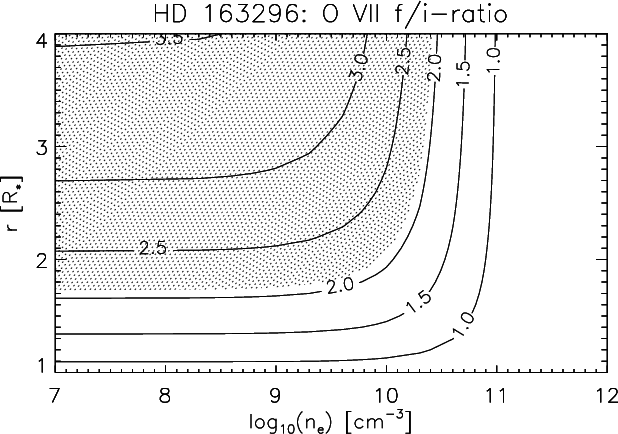
\includegraphics[width=0.5\textwidth]{HD163296_fi}
    \caption{O~{\sc vii} He-like triplet $f/i$ ratio depending on the density of the emitting region and the position. Those regions of the parameter space within the 90\% confidence range are shaded. From: \cite{2009A&A...494.1041G}\label{fig:HDf2i}}
\end{SCfigure}


We will re-analyse XMM-Newton archival data from HD~163296 (the observation is split over two orbits with ObsIDs 0502370201 and 0502370301). The data was originally published by \cite{2009A&A...494.1041G} and is an ideal case to demonstrate our new methods for spectral fitting and answering a real science question at that same time:
\begin{itemize}
    \item Figure~\ref{fig:HDf2i} shows that even a slightly better signal for the $f/i$ line ratio will shrink the confidence region further away from the stellar surface at $R=1\;R_\odot$, ruling out a coronal origin.
    \item In \cite{2009A&A...494.1041G}, the authors were forced to restrict the spectral extraction region to just 66\% of the cross-dispersion profile in the RGS1 (which contains the O~{\sc vii} triplet) because of high background; throwing out one third of the source photons. The gain in signal-to-noise using our new method should be more significant here than in observations where the standard 90\% extraction region was used.
\end{itemize}

From the re-analyzed data, we will measure the $f/i$ ratio with tighter constraints than before and essentially re-do Fig.~\ref{fig:HDf2i} to firmly rule out a coronal origin of the X-ray emission.


\section{Work Plan}
All development and implementation will be done by the funded PI. The unfunded Co-I will provide advice and guidance and test software releases with an estimated effort of about 2 weeks/year. The PI will be responsible for all deliverables and will be the corresponding author on all publications. The PI will also be responsible for the open science and data management plan.

The work plan falls into four work packages.

\subsection{Work package 1: Cross-dispersion profile (4 months)}

We will first address the cross-dispersion profile because this profile can be read from existing XMM-Newton calibration files unlike the background lightcurve, which differs by observation. It is the goal of this proposal to find a practical, tested, and documented method to fit XMM-Newton grating data that takes the cross-dispersion profile into account; we cannot know the best way to implement this before doing the work. We will thus implement three different approaches and systematically compare their performance; time estimates are based on the time we spent to implement our prototype code.

\begin{description}
    \item[Approach 1: 2D fitting:] We will bin the events into a 2D image with axes wavelength and cross-dispersion as in Fig~\ref{fig:rgs1} (left) and Fig.~\ref{fig:toy2d} (left). Sherpa has support for 2D fits, the main task is to implement the 2D model. We will read the cross-dispersion profile from the calibration files and set up a model in Sherpa that folds the model spectrum with the ARF and RMF in 1D and then expands this in the second dimension according to the cross-dispersion profile. (1 month)
    \item[Approach 2: Multiple 1D fits:] We will refine the scripts used in proto-typing and determine reasonable splits of the cross-dispersion profile. We will then adjust the extracted PHA and ARF/RMF files, such that they apply only to certain sub-regions, e.g.\ from 0-50\%, 50-60\%, 60-70\% etc.\ of the cross-dispersion profile. We will fit all the spectra simultaneously, but with the background rates set according to their relative areas. This approach is less granular than the 2D fitting, but can be implemented using current OGIP-style PHA and ARF/RMF files. (1 month)
    \item[Approach 3: Math:] We will work out the mathematics of the problem and see if there is a way to include the cross-dispersion profile in the likelihood function. (1 month)
\end{description}

We will run and debug all three approaches on a few real datasets. We will also systematically explore how well they work depending on the number of source counts and background rate. To do that, we will pick real observations of very bright sources where background is negligible and observations with no source at the aimpoint, so that all detected photons are background events. We can then construct new datasets by drawing photons from either list and thus tune what ratio of source and background counts we want to test, while at the same time reproducing detector characteristics such as increased noise at the chip edges. We will test the performance of different numerical optimizers and experiment with different binning in cross-dispersion direction.

Once we have a working implementation, we will package it, add documentation and tutorials, release it and begin outreach to the community to advertise the method. (1 month)

\objectivebox{Key deliverables}{%
    \begin{itemize}
        \item Release of software package for fitting RGS data with spectral models while taking into account the cross-dispersion profile. The software package will follow best practices for continuous integration and testing.
        \item Documentation of the software package
        \item Tutorials in the form of notebooks and presentations/workshops at a conference
    \end{itemize}
}

\subsection{Work package 2: CCD energy (1 months)}
Filtering in CCD energy is exactly analogous to filtering in the spatial detector direction. We will repeat all steps from work package 1 for the CCD energy direction to get to a 3D fit (wavelength, corss-dispersion, CCD energy). Since we have already implemented the 2D fit, we expect this to be relatively fast.

\objectivebox{Key deliverables}{
    \begin{itemize}
        \item Release new version of software
        \item Update documentation and tutorials
    \end{itemize}
}

\subsection{Work package 3: Background rate (2 months)}
This work package essentially repeats the three approaches from work package 1: Add another dimension to the histogram of detected events to reach a 4D cube (wavelength, cross-dispersion, CCD energy, background rate) or split the data into subsets with different background rates or find a mathematical solution to include the background rate in the likelihood function. Since is this basically a repetition of work package 1 and much of the code will have been implemented in work package 1 already, we expect it to be much faster.

Development of the code will be followed by testing different numerical optimization algorithms and documenting the new additions to the software, recommendations for running it, and updating the tutorials, followed by a third software release.
The method will be published in a peer-reviewed journal. We prefer to publish a pure method paper, but might decide to combine with the fitting and interpretation of the HD~163296 data in work package 4.

\objectivebox{Key deliverables}{
    \begin{itemize}
        \item Release of software package for fitting RGS data with spectral models while taking into account the cross-dispersion profile \emph{and fluctuations in the background rate}.
        \item Updated documentation of the software package
        \item Updated Tutorials
        \item Publication about the software package in a peer-reviewed journal
    \end{itemize}
}

\subsection{Work package 4: Application to HD~163296 (1 month)}

The HD~163296 dataset will be fitted as part of the two previous work packages, so all that remains is to write up the results and submit them for publication.

\objectivebox{Key deliverables}{
    \begin{itemize}
        \item Publication in a peer-reviewed journal about the origin of the soft X-ray emission in HD~163296
    \end{itemize}
}


\subsection{Timeline}
In principle, the work could be done in one year, but we prefer to spread it out over a two-year span to allow for a schedule reserve. For example, when we directly use files from the XMM calibration database, there might be details we need to clarify with the XMM-Newton helpdesk. A back-and-forth of a few emails can easily take two weeks. Similarly, a common wait time for a referee report after paper submission is about 4~weeks initially and 2~weeks for a resubmission. Just those two examples together already sum to two months of hard-to-plan wait time, which can be easily accommodated by distributing the work over two years instead of one.


\section{Open Science and Data Management Plan}
The PI is responsible for the open science and data management.

\subsection{Data}
This proposal works with X-ray data that is already archived by ESA and NASA centers. Despite falling in the category of ``Astrophysical databases'' under the D.2 Astrophysics Data Analysis call, no new raw data is produced in this project; the main product is software. In the course of the data reduction and fitting with the new algorithms intermediate products will be derived (spectra, fitted physical parameters such as densities, temperatures, or elemental abundances). Those data will be included as electronic tables or ``Data behind the figure'' as appropriate in the publications.

\subsection{Software}
During development, we will use Github as our main code repository and will push updates regularly, so that intermediate code is constantly visible to the public. Releases will be synched to Zenodo, which provides long-term archiving and assigns a DOI to each release. We already set up the repository including a code of conduct and guidelines for contributors as part of our proto-typing described in section~\ref{sect:risk}. NASA recommends the use of a permissive open source license. We plan to make all newly developed code available under the MIT license. However, it is good practice in open source to offer any enhancements that might be widely applicable to upstream packages. In our case, we may develop functions, plots, or examples that might be useful to be included into the Sherpa package itself. Sherpa is GLP3 licensed, so any code that we offer to the Sherpa developers as a pull request will also have to be under the GPL3.

In this project, we will develop a relatively small set of Python routines, which we can release as a Python package.

The main product are Jupyter notebooks in Python to show how it all the parts of the analysis fit together using calls to the Python interface to SAS, reading the XMM-Newton calibration database for the cross-dispersion direction, setting up Sherpa/XSPEC spectral models, combined those with the non-spectral dimensions to multi-D models, and fitting in Sherpa, all coupled by Python code. The notebooks we write will contains extensive explanations of each step to allow a user to modify them for their own analysis. We will provide the notebooks both as raw code in the repository for users to copy and modify, and we will also generate rendered HTML versions for easy reading. Since the run time for those notebooks will be long, it is not feasible to re-run them in a continuous integration service with every code change. Instead, we will freeze, release, and archive (to zenodo, with a DOI) the notebooks after major changes to the code base.

NSF funds a cloud environment called SciServer.org \cite{2020A&C....3300412T} that includes a set of containers with SAS and the relevant Python packages already installed (those installations are maintained by NASA HEASARC). SciServer is freely available to the public and provides a Jupyter notebook interface through a webbrowser. We will test that our code works on SciServer and provide instructions how a user can install our package into SciServer to analyze their own datasets without any local installation just through a webbrowser. This way, we open up the science and reduce the barriers for others researchers to use the fitting algorithms developed in this project. This is particularly valuable for teaching, for occasional users, and for those with limited access to modern Linux or Mac hardware.

\subsection{Publications}
All articles will be submitted to AJ/ApJ which are published in full open-access and are indexed in the ADS, consistent with the NASA SMD Open-Source Science Guidance.

%------------------------------------------------
%\phantomsection
%\section*{Acknowledgments} % The \section*{} command stops section numbering

%\addcontentsline{toc}{section}{Acknowledgments} % Adds this section to the table of contents

%So long and thanks for all the fish.

%----------------------------------------------------------------------------------------
%	REFERENCE LIST
%----------------------------------------------------------------------------------------
\newpage
\section{Table of Personnel and Work Effort}

\begin{table}[htb]\small
    \centering
    \caption{Summary of Work Effort (fractional work years)}  \label{tbl:workeffort}
    \begin{tabular}{cclc}\\\hline%\hline
      %
      \multicolumn{1}{c}{Position}&
      \multicolumn{1}{c}{funded}&
      \multicolumn{1}{c}{Year 1}&
      \multicolumn{1}{c}{Year 2}\\\hline
      %
      PI& yes &
      0.33&    0.33\\
      %
      Co-I-1& no &
      0.04 & 0.04\\
    \end{tabular}
  \end{table}

\newpage
\section{Budget Justification}
We request a 2 year duration for the award under the ``small'' ($<$\$125,000/year) costcap. The main expenditure is Personnel time, as provided in the table of Personnel and Work Effort.

In addition to this, we request funds for a laptop computer to develop the analysis code and run it for different datasets in the archive for testing and development, including archival data from HD~163296. Based on our proto-type, we expect to be able to run the fitting on a modern laptop easily, but in development we will try out and compare different numerical fitting algorithms to find which ones perform best. That necessarily means that we will work with algorithms and code packages that will turn out to be inefficient in our use case. Running these experiments on a relatively fast laptop will cut down on development time. We thus price a fairly high-end laptop (14-inch Apple MacBook Pro with M3Max chip), currently listed at \$3200 for our budget estimate.

We request funds for attendance of meetings and conferences. Our main objective is the development of a better method to fit X-ray spectra. Fortunately, more and more astronomers adopt software from sources on-line, but we can reach a bigger audience at an in-person meeting. We conservatively budget two trips: (1)~``X-ray universe'' meeting organized by ESA in support of XMM-Newton. No such meeting has been announced yet for the 2025/2026 time frame, so we budget based on previous meetings in Europe (flight: \$2000, hotel for five nights: \$200/night, conference fee \$500, meals, incidentals etc.\ for a total cost around \$4000). (2)~Another meeting that gathers a lot of potential users of our new algorithms would be the annual meeting of the High-energy division of the AAS. Again based on previous meetings, the cost would be around \$3500 (domestic flights are cheaper, but HEAD meetings are often held in locations with more expensive hotels).

Lastly, we request funding for open-access publishing in AJ/ApJ (currently \$2,651 for an article with 31-50 digital quanta).


\newpage
\phantomsection
\bibliographystyle{unsrtnat}
\setlength\bibsep{0pt}
\bibliography{references}

%---------------------------------------------------------------------------------------

\end{document}